\documentclass[12pt]{mmalatex}
\usepackage{examples}
\usepackage{caption}
\usepackage{pgfplots}

\begin{document}

\section*{Plotting Bessel functions}

\vspace{-5pt}

This simple example uses Mathematica to produce a plot of the first six Bessel functions. Two plots are shown, one created by Mathematica and a second created by LaTeX using the plotting package {\tt\small pgfplots} and the data exported from Mathematica.

\begin{mathematica}
   myData = Partition[Flatten[Table[{x, Table[BesselJ[n, x], {n, 0, 5}]}, {x, 0, 15, 0.1}]], 7];
   myPlot = Plot[Evaluate[Table[BesselJ[n, x], {n, 0, 5}]], {x, 0, 15}, PlotLegends -> "Expressions"];

   Export["example-04-fig.png", myPlot, "PNG"];
   Export["example-04-fig.pdf", myPlot, "PDF"];
   Export["example-04.txt", myData, "Table",  "FieldSeparators" -> " "];
\end{mathematica}

\vfill

\begin{minipage}{\textwidth}
   \centering
   \IfFileExists{example-04-fig.pdf}%
   {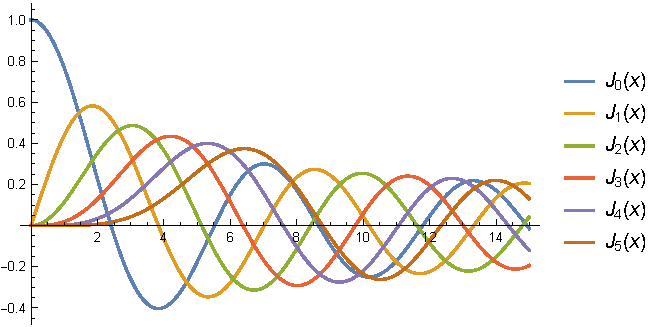
\includegraphics[width=6.4in]{example-04-fig.pdf}}{Failed to create pdf plot.}
   \captionof{figure}{The first six Bessel functions.}
\end{minipage}

\vfill

\clearpage

\pgfplotsset{compat=newest}
\pgfplotsset{width=0.45\textwidth,height=0.34\textwidth}

\subsection*{Using pgfplots}

\begin{minipage}[t]{\textwidth}
   \centering
   \begin{tikzpicture}
      \begin{axis}
         [xmin= 0.0,  xmax=15.0,
          ymin=-0.45, ymax=1.05,
          xlabel=$x$, ylabel=$J_n(x)$,
          grid=major, grid style={dashed,gray!30},
          legend entries = {$J_0$, $J_1$, $J_2$, $J_3$, $J_4$, $J_5$}]
          \addplot[blue]   table [x index=0, y index=1]{example-04.txt};
          \addplot[red]    table [x index=0, y index=2]{example-04.txt};
          \addplot[green]  table [x index=0, y index=3]{example-04.txt};
          \addplot[teal]   table [x index=0, y index=4]{example-04.txt};
          \addplot[orange] table [x index=0, y index=5]{example-04.txt};
          \addplot[purple] table [x index=0, y index=6]{example-04.txt};
      \end{axis}
   \end{tikzpicture}
   \captionof{figure}{The first six Bessel functions.}
\end{minipage}

\vfill

\begin{latex}
   \begin{tikzpicture} % requires \usepackage{pgfplots}
      \begin{axis}
         [xmin= 0.0,  xmax=15.0,
          ymin=-0.45, ymax=1.05,
          xlabel=$x$, ylabel=$J_n(x)$,
          grid=major, grid style={dashed,gray!30},
          legend entries = {$J_0$, $J_1$, $J_2$, $J_3$, $J_4$, $J_5$}]
          \addplot[blue]   table [x index=0, y index=1]{example-04.txt};
          \addplot[red]    table [x index=0, y index=2]{example-04.txt};
          \addplot[green]  table [x index=0, y index=3]{example-04.txt};
          \addplot[teal]   table [x index=0, y index=4]{example-04.txt};
          \addplot[orange] table [x index=0, y index=5]{example-04.txt};
          \addplot[purple] table [x index=0, y index=6]{example-04.txt};
      \end{axis}
   \end{tikzpicture}
   \captionof{figure}{The first six Bessel functions.} % requires \usepackage{caption}
\end{latex}

\end{document}
